\documentclass{report}

\usepackage[utf8]{inputenc}
\usepackage[T1]{fontenc}
\usepackage[french]{babel}
\usepackage{eurosym}
\usepackage[left=2.5cm,right=2.5cm,bottom=2.5cm,top=2.5cm]{geometry}
\usepackage{hyperref}
\usepackage{graphicx}
\usepackage{amsmath}

\begin{document}
\section{Introduction}
Dans ce projet, nous allons chercher à simuler des variables aléatoires. Bien sûr, il est impossible de créer du hasard avec un ordinateur, mais nous allons tenter de nous en rapprocher. Nous allons procéder pas à pas, tout d'abord, nous allons coder un algorithme de base : la simulation d'une variable aléatoire suivant une loi uniforme. A partir de cela, nous allons pour constuire des algorithmes plus complexes permettant de simuler différentes lois. 

\section{Loi uniforme}

Pour comprendre la base de notre projet, nous décidons de coder l'algorithme de base : la simulation d'une variable aléatoire suivant une loi uniforme. Le principe est le suivant : nous allons générer une suite 
\smash{$(x_{n})$} telle que 
$$
\left\{
    \begin{array}{ll}
        x_{0} \in R \\
        x_{n} = ax_{n-1} + c,  \forall n \in N \\
    \end{array}
\right.
$$
On posera un $m$ très grand tel que $\forall n \in N, x_{n} \le m$
. Ensuite, nous divisons tous les termes de la suite par m, ainsi nous obtenons la suite \smash{$(u_{n})$}
 dont tous les termes sont compris entre 0 et 1.

Plusieurs points sont à régler, tout d'abord il faut s'assurer que notre suite \smash{$(u_{n})$} génère des variables uniformément réparties sur $[0;1]$. Pour cela, nous avons choisit des paramètres grâce à des méthodes déjà implémentées et vérifiées. Nous avons trouvé nos paramètres sur  
\href{https://en.wikipedia.org/wiki/Linear_congruential_generator}{cette page}
Nous nous assurons tout de même que notre algorithme est fiable, en vérifiant que pour un grand nombre de données, elles sont bien réparties uniformément sur $[0;1].$ 
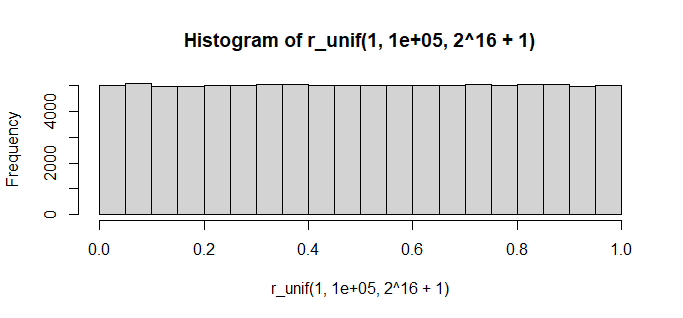
\includegraphics[scale=0.75]{plot_r_unif.png}

Il reste à régler le problème de la "seed", c'est-à-dire notre graîne, le \smash{$(x_{0})$}
 qui démarre la série \smash{$(x_{n})$}
. En effet, si nous ch


\end{document}
						
					